\documentclass[tikz,margin=2mm]{standalone}
\usetikzlibrary{positioning}
\usetikzlibrary{arrows.meta, shapes, calc}

\begin{document}

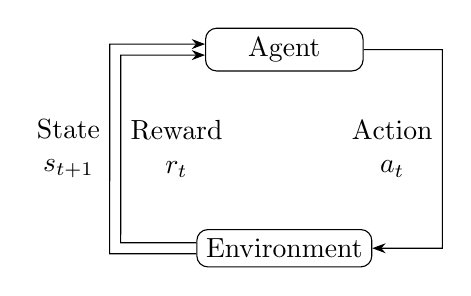
\begin{tikzpicture}[>=Stealth, node distance=2cm]

    % Nodes
    \node[draw, rounded corners, minimum width=2cm] (agent) {Agent};
    \node[draw, rounded corners, minimum width=2cm, below=of agent] (env) {Environment};

    % Arrows and labels
    \draw[->] (agent.east) -- ++(1,0)  -- ($ (env.east) + (0.89,0) $) node[midway, left, align=center] {Action \\ $a_t$} |- (env.east);
    \draw[->] ($ (env.west) + (0,0.07) $) -- ++(-0.96,0) -- ($ (agent.west) + (-1.07,-0.07) $) node[midway, right, align=center] {Reward \\ $r_t$}  |- ($ (agent.west) + (0,-0.07) $) ;
    \draw[->] ($ (env.west) + (0,-0.07) $) -- ++(-1.1,0) -- ($ (agent.west) + (-1.21,+0.07) $) node[midway, left, align=center] {State \\ $s_{t+1}$}  |- ($ (agent.west) + (0,+0.07) $) ;

\end{tikzpicture}


\end{document}
